% !TEX TS-program = pdflatexmk
% !BIB TS-program = bibtex

\documentclass[12pt, a4paper, twoside]{book}
\usepackage{import}
\subimport{../}{preamble}
\ExecuteBibliographyOptions{articletitle=false}
\standalonetrue
\onehalfspacing
\begin{document}

\begin{singlespace}
\color{white}\chapter{Plasmon Interactions in Tip Dimers}
\label{ch:tip_interactions}
\end{singlespace}

\AddToShipoutPictureBG*{ \AtPageUpperLeft{ \put(0,-240)
{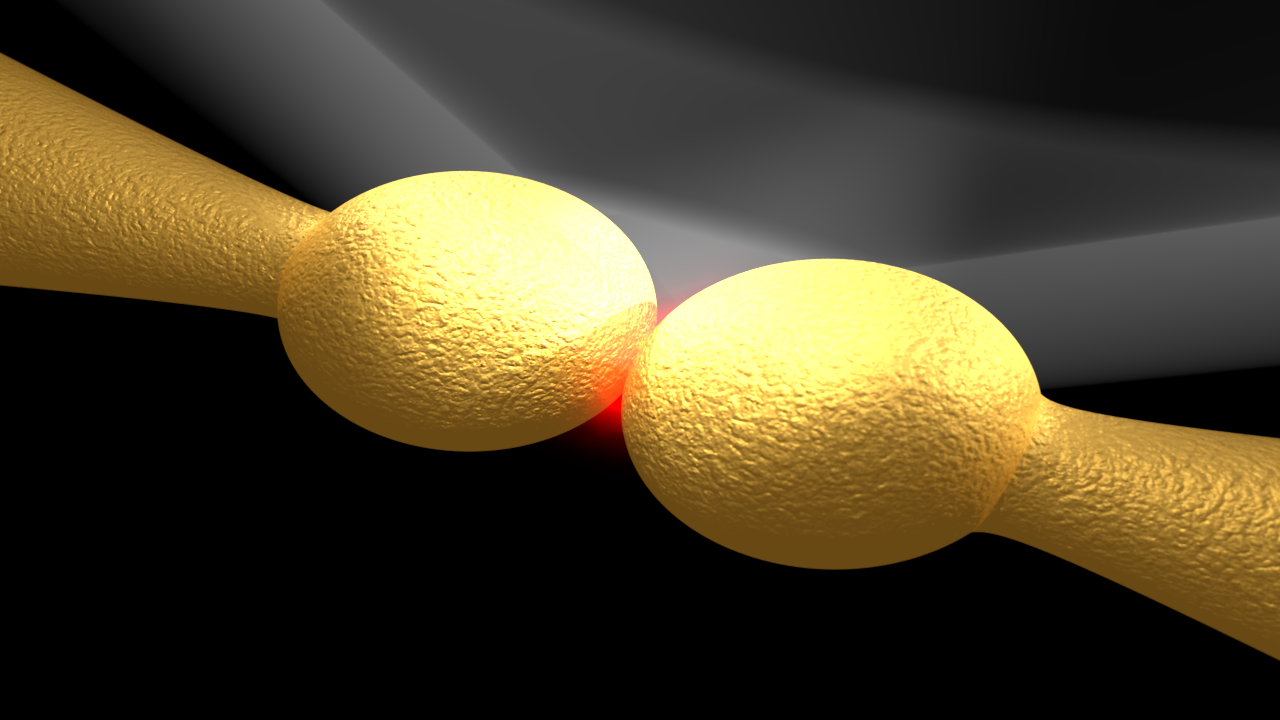
\includegraphics[width=\paperwidth, clip=true, trim=0 80 0 100]{figures/chapter_cover.png}}
}}

The final set of experiments discussed in this thesis are the product of each of the developments from the previous chapters, utilising pairs of tips in the microscope platform to investigate the limits of plasmon coupling. Coupling between different tip morphologies is dynamically investigated to both confirm plasmonic behaviour in tips and increase understanding of the characteristic regimes of plasmon coupling. Through this work an improved interpretation of future results in sub-nm plasmonic gaps can be attained, along with insight into the mechanisms by which TENOM operates.

\subimport{./}{tip_dimer_interactions}
\subimport{./}{quantum_effects}

\section{Conclusions}

Multiple different combinations of tips in a dimer configuration are used to probe plasmon coupling. Sharp Au tips exhibit no obvious plasmon resonances under far-field illumination and no gap mode coupling is observed with other sharp or spherical Au tips. This is caused by the lack of an antenna-like geometry in sharp tips. Plasmons excited at the apex of spherical Au tips, on the other hand, interact and hybridise. The behaviour of these modes is as expected, with similarity to plasmons in AuNP dimers. The inherent asymmetry between the large spherical tip structures leads to more complex scattering spectra wherein anti-bonding modes are no longer dark. Their evolution into gap modes is something not previously seen before in a single dynamic system.

To conclude experimental work, tip dimers are used to determine the influence of quantum effects, specifically forms of quantum charge transport, on plasmon coupling in sub-nm gaps. Using this approach, the development of a charge transfer plasmonic regime is dynamically observed as classical plasmon hybridisation is heavily screened. Critical conductances are estimated for each domain change using direct correlations between optical spectra and current measurements, showing agreement with theoretical principles. Though no quantitative measurements, such as temperature, voltage or power dependences, are made to guarantee that charge transfer is via quantum tunnelling and ballistic transport, these are the most likely mechanisms. Further investigation could quantify this, although sub-nm gap phenomena are not expected to depend on the conduction mechanism. Comparison with tip dimers coated in different molecular layers of varying conductivities would also further understanding into the effects of charge transfer in plasmonic systems and forms the basis of future experiments on this topic.

In summary, the existence of two distinct regimes of quantum charge transport have been detected in sub-nm plasmonic cavities. These are:
\begin{itemize}
\item The crossover regime (also known as the tunnelling regime), wherein electrons tunnelling through the barrier screen the capacitive interaction between opposite gap surfaces, reducing plasmon coupling strength and slowing coupling to a halt.
\item The conductive regime, where strong currents at \G0-level conductances heavily attenuate hybridised plasmons leading to the previously observed blueshift transition into charge transfer plasmons.
\end{itemize}
Though numerous theoretically predictions have been in recent years, this is the first time that correlated experimental measurements between plasmon resonances and conductance have been performed.

\ifstandalone
\begin{singlespace}
\fontsize{8pt}{1em}\selectfont
\printbibliography[notcategory=fullcited]
\end{singlespace}
\fi

\end{document}